\chapter{Secure bootloader} % Grammarly OK
\label{custom_bootloader}

Bootloaders are used for direct memory manipulation and usually run before the user's application, e.g., an operating system. It is highly processor and board specific. The term “bootloader” is a shortened form of the words “bootstrap loader”. The term stems from the fact that the boot manager is the key component in starting up the computer, so it can be likened to the support of a bootstrap when putting a boot on \citep{bootloader_intro}. \autoref{appendix_cmd_ref_bootloader} contains commands reference for the bootloadder.

\section{Developed bootloader overview}

The developed bootloader can be controlled using a command shell communication over UART. The bootloader can load new applications over UART. Also, many memory management functions are added. When updating the application bootloader accepts three types: binary (.bin), Intel hex (.hex) or Motorola S-record (.srec). A transmitted new application can additionally be checksummed with SHA256 or cyclic redundancy check (CRC32).

The default STM32F407 microcontroller's bootloader doesn't allow the aforementioned functionality and that is the main motivation for writing code for this platform \citep{stm32f407_ref_man}. The first version of the bootloader is developed for the STM32F407-Discovery board. Bootloader code is situated in the first three sectors of microcontrollers memory, as seen in \autoref{tab:bootloader_flash}. The fourth section is used as persistent memory (not loaded on the code startup) for communication between the bootloader and the user's application. More about application boot record in \autoref{boot_record}. The bootloader is written according to the BARR:C-2018 C coding standard to minimize defects in code \citep{barr_c}. The file structure of the bootloader source code for STM32F407 is as follows:
\begin{figure}[H]
\dirtree{%
.1 /.
.2 Core - Hardware initialization code and main.c.
.2 Drivers - STM's HAL Driver.
.2 custom\textunderscore bootloader - Source code of the custom bootloader. 
.3 commands.
.4 cbl\textunderscore cmds\textunderscore etc.c/.h.
.4 cbl\textunderscore cmds\textunderscore memory.c/.h.
.4 cbl\textunderscore cmds\textunderscore opt\textunderscore bytes.c/.h.
.4 cbl\textunderscore cmds\textunderscore template.c/.h.
.4 cbl\textunderscore cmds\textunderscore update\textunderscore act.c/.h.
.4 cbl\textunderscore cmds\textunderscore update\textunderscore new.c/.h.
.3 etc.
.4 cbl\textunderscore boot\textunderscore record.c/.h.
.4 cbl\textunderscore checksum.c/.h.
.4 cbl\textunderscore common.c/.h.
.3 custom\textunderscore bootloader.c.h.
.2 custom\textunderscore bootloader\textunderscore system - HAL for the custom bootloader. 
.2 startup - Contains assembly file for a startup. 
.2 third\textunderscore party.
.3 sha256 - Used for checksum when loading a new file. 
}
\caption{Bootloader file structure for STM32F4007 microcontroller}
\label{tree:bootloader}
\end{figure}

\section{Architecture of the bootloader}

Bootloader architecture is simple. On entry, the bootloader checks if the blue button on the discovery board is pressed, if it is pressed bootloader is skipped and the user's application starts. The bootloader starts otherwise. When the bootloader starts, it checks if the user's application update is needed and updates it if needed. The next step is going into the system state machine.

The bootloader has 3 states: Operation, error and exit. Operation state flow is shown in \autoref{fig:bootloader_flow}. Operation state waits for incoming commands and processes them, error state constructs and sends an error message back to the user. Exit state is called right before exiting, it is used to deconstruct data from the bootloader.



\begin{figure}[H]
    \centering
    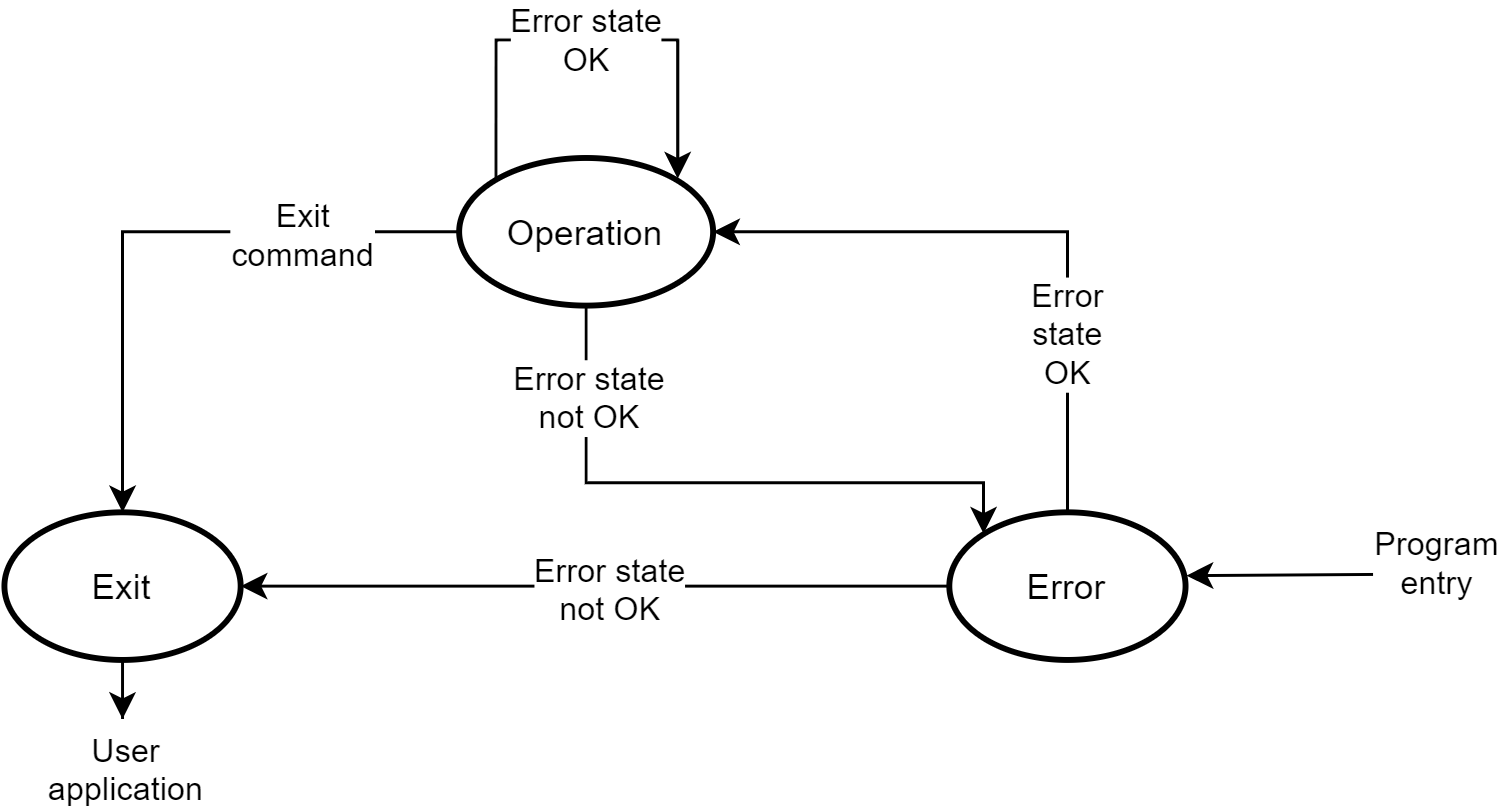
\includegraphics[width=.8\linewidth]{images/bootloader_flow.png}
    \captionof{figure}{State machine of the bootloader}
    \label{fig:bootloader_flow}
\end{figure}

\begin{figure}[H]
    \centering
    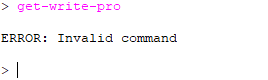
\includegraphics[width=.4\linewidth]{images/bootloader_cmd_err.png}
    \captionof{figure}{Example of an error from error state}
    \label{fig:bootloader_cmd_err}
\end{figure}

\section{Flash memory organization}

When using the bootloader the flash module is organized a shown in \autoref{tab:bootloader_flash}. 

\begin{table}[H]
\begin{tabular}{lllll}
\textbf{Block} & \textbf{Used by} & \textbf{Name} & \textbf{Block base addresses} & \textbf{Size} \\
 & \cellcolor[HTML]{D9D9D9} & \cellcolor[HTML]{D9D9D9}Sector   0 & \cellcolor[HTML]{D9D9D9}0x0800   0000 - 0x0800 3FFF & \cellcolor[HTML]{D9D9D9}16   Kbytes \\
 & \cellcolor[HTML]{D9D9D9} & \cellcolor[HTML]{D9D9D9}Sector   1 & \cellcolor[HTML]{D9D9D9}0x0800   4000 - 0x0800 7FFF & \cellcolor[HTML]{D9D9D9}16   Kbytes \\
 & \multirow{-3}{*}{\cellcolor[HTML]{D9D9D9}Bootloader} & \cellcolor[HTML]{D9D9D9}Sector   2 & \cellcolor[HTML]{D9D9D9}0x0800   8000 - 0x0800 BFFF & \cellcolor[HTML]{D9D9D9}16   Kbytes \\
 & Boot record & Sector   3 & 0x0800   C000 - 0x0800 FFFF & 16   Kbytes \\
 & \cellcolor[HTML]{D9D9D9} & \cellcolor[HTML]{D9D9D9}Sector   4 & \cellcolor[HTML]{D9D9D9}0x0801   0000 - 0x0801 FFFF & \cellcolor[HTML]{D9D9D9}64   Kbytes \\
 & \cellcolor[HTML]{D9D9D9} & \cellcolor[HTML]{D9D9D9}Sector   5 & \cellcolor[HTML]{D9D9D9}0x0802   0000 - 0x0803 FFFF & \cellcolor[HTML]{D9D9D9}128   Kbytes \\
 & \cellcolor[HTML]{D9D9D9} & \cellcolor[HTML]{D9D9D9}Sector   6 & \cellcolor[HTML]{D9D9D9}0x0804   0000 - 0x0805 FFFF & \cellcolor[HTML]{D9D9D9}128   Kbytes \\
 & \multirow{-4}{*}{\cellcolor[HTML]{D9D9D9}\begin{tabular}[c]{@{}l@{}}Current\\ application\end{tabular}} & \cellcolor[HTML]{D9D9D9}Sector   7 & \cellcolor[HTML]{D9D9D9}0x0806   0000 - 0x0807 FFFF & \cellcolor[HTML]{D9D9D9}128   Kbytes \\
 &  & Sector   8 & 0x0808   0000 - 0x0809 FFFF & 128   Kbytes \\
 &  & Sector   9 & 0x080A   0000 - 0x080B FFFF & 128   Kbytes \\
 &  & Sector   10 & 0x080C   0000 - 0x080D FFFF & 128   Kbytes \\
\multirow{-12}{*}{Main   memory} & \multirow{-4}{*}{\begin{tabular}[c]{@{}l@{}}New\\    \\ application\end{tabular}} & Sector   11 & 0x080E   0000 - 0x080F FFFF & 128   Kbytes \\
\rowcolor[HTML]{D9D9D9} 
\multicolumn{3}{l}{\cellcolor[HTML]{D9D9D9}System memory} & 0x1FFF   0000 - 0x1FFF 77FF & 30   Kbytes \\
\rowcolor[HTML]{D9D9D9} 
\multicolumn{3}{l}{\cellcolor[HTML]{D9D9D9}OTP area} & 0x1FFF   7800 - 0x1FFF 7A0F & 528   bytes \\
\rowcolor[HTML]{D9D9D9} 
\multicolumn{3}{l}{\cellcolor[HTML]{D9D9D9}Option bytes} & 0x1FFF   C000 - 0x1FFF C00F & 16   bytes
\end{tabular}
\caption{STM32F407 flash memory organization}
\label{tab:bootloader_flash}
\end{table}


\section{Application boot record}
\label{boot_record}

Application boot record is used to store metadata about the current user's application and new user's application. Metadata consists of: 
\begin{itemize}
    \item Checksum used for transmission,
    \item Application type used while transmitting,
    \item Length of application during transmission.
\end{itemize}
The boot record is also used to signalize that update of the application is needed to the bootloader. The flag is set when a new application is successfully transmitted.

\autoref{memory_areas} and \autoref{app_boot_rec} show modifications added to the linker file needed to add the boot record. Address 0x800C000 is the starting address of sector 3 of the flash memory.

\begin{lstlisting}[frame=single, label={memory_areas}, caption={Memory areas from the linker file.}, captionpos=b]
/* Specify the memory areas */
MEMORY
{
RAM (xrw)      : ORIGIN = 0x20000000, LENGTH = 128K
CCMRAM (rw)      : ORIGIN = 0x10000000, LENGTH = 64K
/* Allow bootloader only first 3 sectors */
FLASH (rx)      : ORIGIN = 0x8000000, LENGTH = 48K 
/* Allow sector 3 for app boot record */
SEC3 (rx)		: ORIGIN = 0x800C000, LENGTH = 16K
}
\end{lstlisting}

\begin{lstlisting}[frame=single, label={app_boot_rec}, caption={Application boot record from the linker file.}, captionpos=b]
  /* Application boot record */
  .appbr 0x800C000 (NOLOAD):
  {
    . = ALIGN(4);
    _sappbr = .;       
    *(.appbr)
    *(.appbr*)
    
    . = ALIGN(4);
    _eappbr = .;   
  } >SEC3
\end{lstlisting}


\section{User application modifications}

At the start of every STM32F407 program is a vector table. The vector table contains numerous interrupt and exception vectors. List of all vectors is available in \citep[p.~372]{stm32f407_ref_man}. On startup the program calls the vector on the address 4, the name of that vector is fittingly Reset handler. But before calling the reset handler main stack pointer(MSP) is set from the address 0. 

Because the program expects the main stack pointer and resets handler vector to be on the start of the program vector offset register (VTOR) is available. The vector offset register is simply added onto the flash memory base address to allow multiple programs in the same flash memory. Perfect for writing a bootloader!

To sum up, before the bootloader jumps to the user application it must set the MSP to one of the user's application then it jumps to the application's reset handler. A vector offset register can be set by the bootloader or in the user's application, former is chosen in this project.

